
\documentclass[10pt]{beamer}
\usepackage{verbatim}
\mode<presentation> {
	\usetheme{Madrid}
}

\usepackage{graphicx}
\usepackage{booktabs}

\title[Lettori-Scrittori]{Problema dei lettori-scrittori}
\subtitle{Problema e possibili soluzioni}
\author{Francesco Lucia}
\institute[]
{
	Università degli studi della Basilicata \\
	\medskip
}
\date{A.A. 2021/2022}

\begin{document}
	
	\begin{frame}
		\titlepage
	\end{frame}
	\begin{frame}
		\frametitle{Il Problema}
		
		Il problema dei lettori-scrittori è un classico problema di concorrenza e sincronizzazione che analizza uno scenario che si verifica in molti programmi applicativi.
		
		Nel problema si ha un dato condiviso (che può essere un file, una variabile, un database, un'area di memoria) e una serie di processi che vogliono accedervi in modalità di scrittura o lettura. I processi che chiameremo "lettori" intendono leggere il contenuto condiviso, i processi "scrittori" intendono modificarlo.
	
		La differenza con un problema di sincronizzazione classico è nel fatto che è possibile differenziare le strategie da adottare in base al tipo di processo che accede alla risorsa ottimizzando la soluzione.
	\end{frame}

\begin{frame}
	\frametitle{Analisi del problema}
	
	Infatti se i processi lettori leggessero contemporaneamente ad un processo scrittore, potrebbero leggere solo una parte del contenuto o non riuscire ad accedervi affatto. Se due scrittori scrivessero contemporaneamente potrebbero sovrascrivere uno il lavoro dell'altro o generare dati corrotti.\\Mentre se due lettori dovessero leggere contemporaneamente non si verificherebbe alcun problema.
	
	Analizzando il problema si possono quindi riassumere una serie di considerazioni:
	
	\begin{itemize}
		\item Più lettori possono leggere contemporaneamente i dati.
		\item Se uno scrittore sta scrivendo, nessun processo può leggere.
		\item Solo uno scrittore per volta può scrivere.
	\end{itemize}

	La soluzione si serve di strutture per regolare l'accesso alla risorsa imponendo che siano rispettate le 3 considerazioni appena fatte.
\end{frame}

%--- SOLUZIONE IN C ---%

\begin{frame}[fragile]
	\frametitle{Creazione di lettori e scrittori}
	Nell'implementare la soluzione sono stati creati 12 threads lettori e 7 threads scrittori con l'utilizzo della libreria pthreads. Questa permette di avviare un thread con la sintassi
	\begin{verbatim}
		int  pthread_create(pthread_t  *thread,
		const  pthread_attr_t*  attr, void  *(*start_routine)(void*)
		, void*  arg  );
	\end{verbatim}
	Che prende come parametri il riferimento al descrittore del thread (che contiene il thread\_id), un puntatore alla struttura (attr) con le caratteristiche del thread, la funzione eseguita dal thread e il puntatore ai parametri da passare alla funzione.
	\\In questo caso per la creazione degli scrittori è sufficiente l'istruzione 
	\begin{verbatim}
		pthread_create(&scrittori[i], NULL, scrittore, (void*)i);
	\end{verbatim}
	Dove l'array scrittori è stato creato precedentemente con l'istruzione
	\begin{verbatim}
		pthread_t scrittori[NUMERO_SCRITTORI];
	\end{verbatim}
\end{frame}

\begin{frame}[fragile]
	\frametitle{Soluzione con semafori e lock mutex}
	Per semplicità nella soluzione proposta la memoria condivisa è rappresentata da una semplice variabile con visibilità globale, inizialmente con valore 1.
	\\I lettori non fanno altro che stampare il contenuto della variabile sullo schermo, gli scrittori invece modificano la variabile moltiplicandone il contenuto per un numero casuale tra 1 e 10, con l'istruzione
	\begin{verbatim}
		variabile_condivisa *= rand()%10+1;
	\end{verbatim}
	A causa della semplicità delle operazioni di lettura e scrittura (trattandosi di una sola variabile), le operazioni vengono effettuate istantaneamente dai threads alla loro creazione. Per simulare una casualità la prima istruzione di un thread è una sleep con un parametro generato casualmente tra 0 e 3 secondi dalla funzione \emph{float randomFloat(float min, float max)}
\end{frame}

\begin{frame}[fragile]
	\frametitle{Soluzione con semafori e lock mutex}
	La soluzione privilegia i lettori.
	La variabile \emph{num\_lettori} conta i lettori attualmente attivi. La sincronizzazione è gestita attraverso l'utilizzo in un lock mutex (\emph{mutex}) per la sezione critica relativa all'aggiornamento della variabile contatore dei lettori, e un semaforo (\emph{semaforo\_scrittura}) per regolare l'autorizzazione a scrivere per gli scrittori.
	
	Il problema della soluzione è la possibilità di starvation per gli scrittori, se infatti ci sono uno o più lettori attivi e continuano ad arrivarne altri, il programma darà precedenza a questi autorizzando lo scrittore a scrivere solo nel momento in cui tutti i lettori avranno terminato.
	
	Per ovviare al problema si potrebbero implementare dei sistemi che mettano un limite al tempo che uno scrittore può attendere, andando a sospendere le operazioni di lettura per consentire di smaltire la coda degli scrittori.
\end{frame}

\begin{frame}[fragile]
	\frametitle{Soluzione con semafori e lock mutex}
	\begin{columns}
		\begin{column}{0.4\textwidth}
			Lock Mutex
			
			Variabile booleana, un processo acquisisce il lock e il successivo che tenta di acquisirlo rimane in attesa finché il primo non lo rilascia.
			
			\begin{verbatim}
				acquire() {
					while (!available) ;
					available = false;
				}
				release() {
					available = true;
				}
			
		\end{verbatim}
		\end{column}
		\begin{column}{0.4\textwidth}
			Semaforo
			
			Variabile intera o booleana, un processo acquisisce il semaforo e i successivi in attesa vengono inseriti in una coda dei processi
			
			\begin{verbatim}
				wait(semaphore *S) {
					S->value--;
					if (S->value < 0) {
						aggiungi il processo a S->list;
						sleep();
					}
				}
				signal(semaphore *S) {
					S->value++;
					if (S->value <= 0) {
						togli un processo P da S->list;
						wakeup(P);
					}	
				}
			\end{verbatim}
		\end{column}
	\end{columns}
\end{frame}


\begin{frame}[fragile]
	\frametitle{Soluzione con semafori e lock mutex}
		Il lock mutex utilizza il tipo \emph{pthread\_mutex} di pthread. Un thread può acquisire il lock su un lock mutex prima di entrare in una sezione critica e successivamente rilasciarlo con le procedure pthread\_mutex\_lock(\&mutex) e pthread\_mutex\_unlock(\&mutex).
		
		I semafori sono implementati nella libreria \emph{semaphore.h}, un semaforo di tipo \emph{sem\_t} può essere inizializzato con la procedura \emph{sem\_init(\&semaforo,0, 1)}, dove 0 indica che il semaforo è condiviso solo nei threads del processo che l'ha generato, il terzo parametro (1) è il valore iniziale del semaforo.
		
		Le istruzioni per acquisire e rilasciare il semaforo sono rispettivamente \emph{sem\_wait(\&semaforo)} e \emph{sem\_post(\&semaforo)}
\end{frame}
	
	\begin{frame}[fragile]
		\frametitle{Il codice}
		\begin{columns}
			\begin{column}{0.3\textwidth}
				
				\begin{figure}
					\centering
					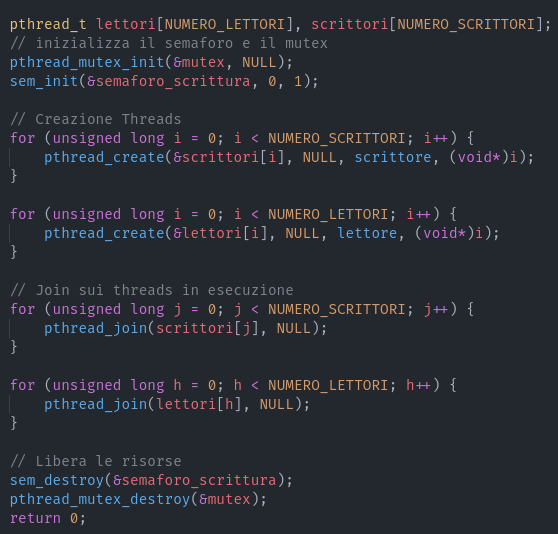
\includegraphics[width=2\linewidth]{img/main}
				\end{figure}
				
			\end{column}\hspace{100pt}
			\begin{column}{0.3\textwidth}
				Metodo main
				
				Dopo l'inizializzazione del semaforo e del mutex, due cicli for creano i threads per gli scrittori e i lettori, poi con \emph{pthread\_join} attenda che questi terminino.
				
				Successivamente è importante deallocare le risorse (terzultima e penultima riga), dimenticarsene potrebbe causare perdita di memoria in alcune situazioni.
			\end{column}
		\end{columns}
	\end{frame}

\begin{frame}[fragile]
	\frametitle{Il codice}
			
			\centering
			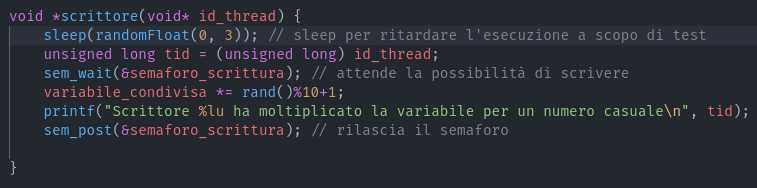
\includegraphics[width=\linewidth]{img/scrittore}
			Lo scrittore chiama una \emph{sem\_wait} sul semaforo, una volta acquisito modifica la variabile e stampa la scritta di logging, poi chiama una \emph{sem\_post} per liberare il semaforo e permette ad altri scrittori/lettori di agire.
\end{frame}

\begin{frame}[fragile]
	\frametitle{Il codice}
		\begin{columns}
		\begin{column}{0.3\textwidth}
			
			\begin{figure}
				\centering
				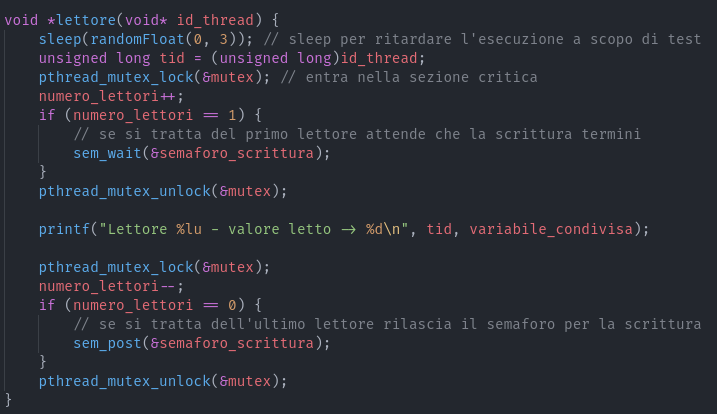
\includegraphics[width=2\linewidth]{img/lettore}
			\end{figure}
			
		\end{column}\hspace{100pt}
		\begin{column}{0.3\textwidth}
			Il lettore acquisisce il lock sul mutex, incrementa la variabile che conta il numero di lettori attualmente attivi, se è il primo lettore (if) acquisisce il semaforo\_scrittura (assicurandosi così che non ci siano processi che stanno scrivendo), rilascia poi il lock sul mutex in modo da permettere ad altri lettori di leggere contemporaneamente e legge il valore.
		\end{column}
	\end{columns}
	
\end{frame}
\begin{frame}[fragile]
	\frametitle{Il codice}
	\begin{columns}
		\begin{column}{0.3\textwidth}
			
			\begin{figure}
				\centering
				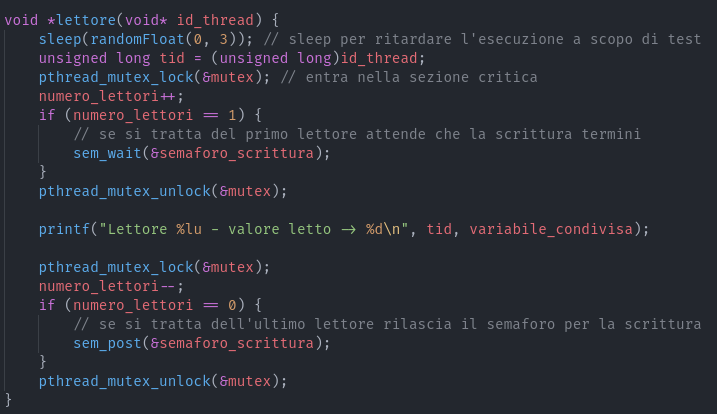
\includegraphics[width=2\linewidth]{img/lettore}
			\end{figure}
			
		\end{column}\hspace{100pt}
		\begin{column}{0.3\textwidth}
		Dopo la lettura riacquisisce il lock sul mutex per decrementare la variabile numero\_lettori, se non ci sono più processi che stanno leggendo rilascia il semaforo\_scrittura per permettere ad uno scrittore di iniziare.
		
		Successivamente rilascia il lock sul mutex
		\end{column}
	\end{columns}
	
\end{frame}
	%--- Esecuzione C ---%
	\begin{frame}[fragile]
		\frametitle{Prima esecuzione}
		\begin{figure}
			\centering
			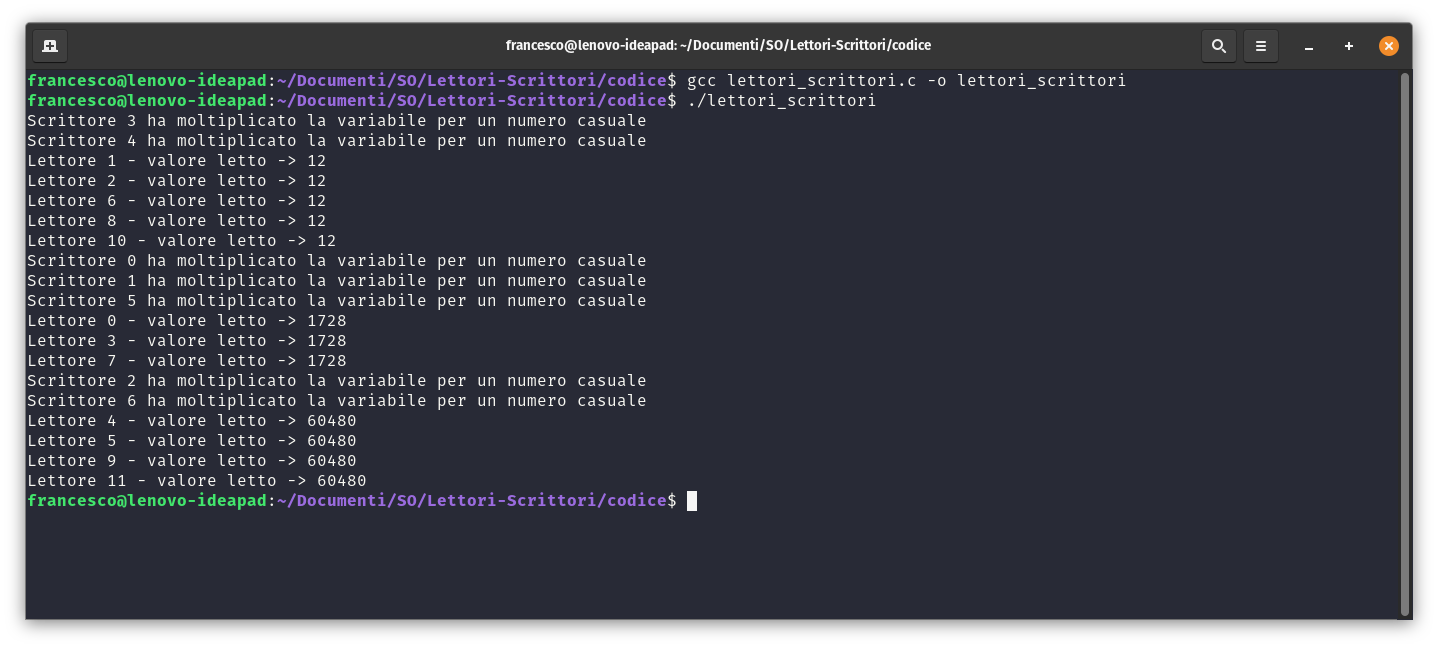
\includegraphics[width=1.03\linewidth]{img/esecuzione/programC1}
			\label{fig:programc1}
		\end{figure}
	\end{frame}
	\begin{frame}[fragile]
		\frametitle{Seconda esecuzione}
		\begin{figure}
			\centering
			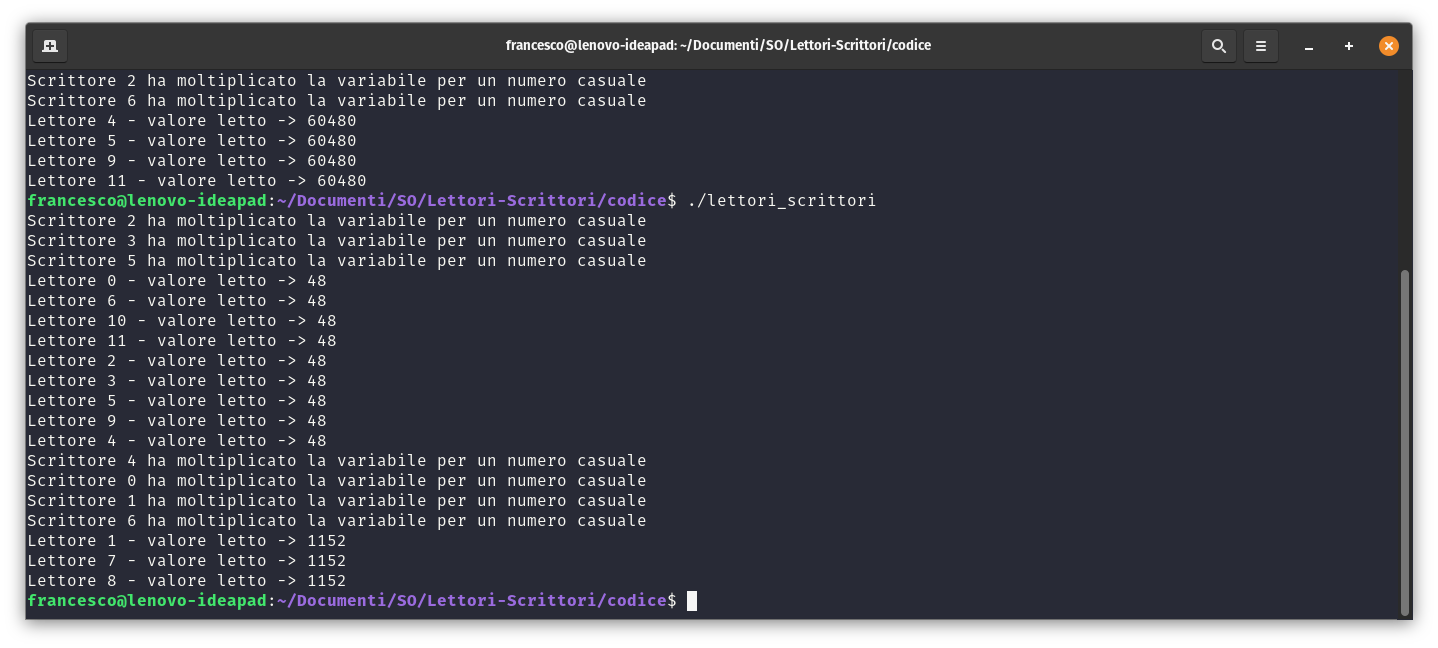
\includegraphics[width=1.03\linewidth]{img/esecuzione/programC2}
			\label{fig:programc1}
		\end{figure}
	\end{frame}

%--- SOLUZIONE IN JAVA ---%

\begin{frame}
	\frametitle{Monitor}
	L'uso dei semafori in alcune situazioni è macchinoso e necessita di uno sforzo particolare da parte dello sviluppatore. Un errore logico può causare bug che si manifestano solo in condizioni particolari e pertanto difficili da individuare.
	
	Un monitor è un tipo di dato che incapsula la logica di gestione della sincronizzazione, esponendo delle funzioni utilizzabili dagli sviluppatori nei programmi che slegano la singola operazione dalla logica di sincronizzazione.
	
	Il secondo esempio di implementazione è una soluzione in linguaggio Java che utilizza una classe Monitor per mostrare come questa semplifichi poi la gestione dei lettori e scrittori (e di conseguenza il codice).
\end{frame}

\begin{frame}
	\frametitle{Soluzione con Monitor}
	La classe \emph{Memoria} non fa altro che mantenere lo stato della memoria condivisa tra i threads, espone i metodi scrivi e leggi.
	
	La classe \emph{LettoriScrittori} contiene il main del programma, si occupa di creare gli oggetti monitor e memoria e di avviare i threads (la struttura del programma è simile a quella vista per la prima soluzione con le dovute differenze sintattiche e nelle librerie utilizzate per l'avvio dei threads).
	
	Le classi \emph{Lettore} e \emph{Scrittore} estendono la classe astratta \emph{Thread} (metodo standard per la creazione di thread in java), nel metodo \emph{run()} svolgono le operazioni di lettura/scrittura, con la semplice accortezza di chiamare (prima e dopo l'accesso alla risorsa) i rispettivi metodi della classe monitor \emph{iniziaLettura()}/\emph{terminaLettura()} e \emph{iniziaScrittura()}/\emph{terminaScrittura()}.
\end{frame}

\begin{frame}
	\frametitle{Classe Lettore}
		\begin{figure}
			\centering
			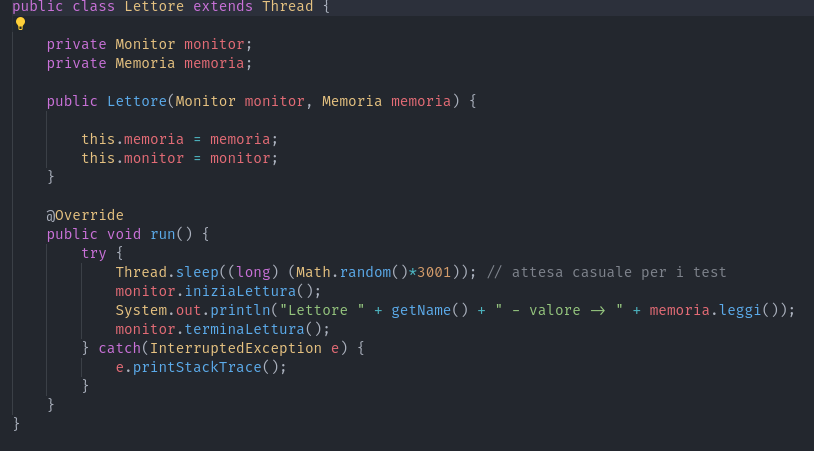
\includegraphics[width=\linewidth]{img/lettore_java}
		\end{figure}
\end{frame}
\begin{frame}
	\frametitle{Classe Scrittore}
	\begin{figure}
		\centering
		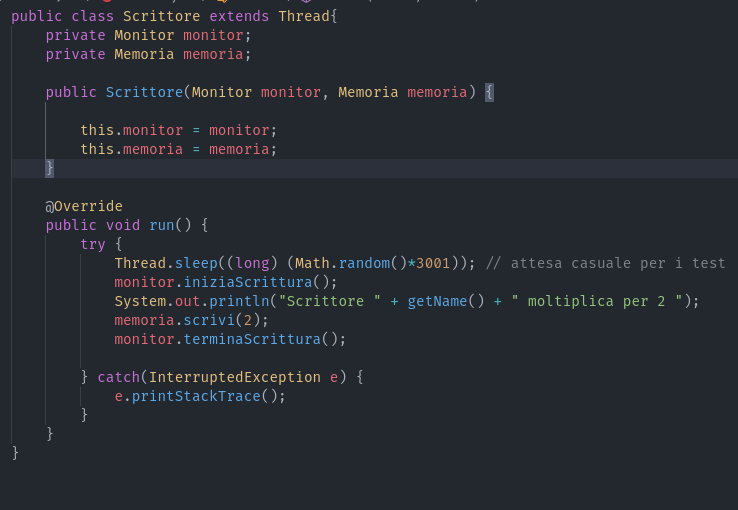
\includegraphics[width=\linewidth]{img/scrittore_java}
	\end{figure}
\end{frame}

\begin{frame}
	\frametitle{Sincronizzazione in Java}
	Il locking è gestibile in Java con i lock rientranti (\emph{ReentrantLock}) che svolge nel Monitor funzioni analoghe al lock mutex nell'implementazione in C. I metodi per acquisire e rilasciare il lock sono rispettivamente \emph{lock()} e \emph{unlock()}.
	
	Le variabili condizionali sono associate a un lock, il metodo \emph{newCondition()} chiamato sul riferimento ad un oggetto \emph{ReentrantLock} crea un nuovo oggetto di tipo \emph{Condition}, che espone i metodi \emph{wait()} e \emph{signal()}.
	
	All'interno della classe Monitor troviamo diversi contatori che mantengono informazioni lo stato degli accessi alle risorse: \emph{numeroLettori}, \emph{numeroScrittori}, \emph{lettoriInAttesa}, \emph{scrittoriInAttesa}.
	
	La classe Monitor utilizza un \emph{ReentrantLock} per gestire le sezioni critiche per l'aggiornamento dei contatori e due variabili condition \emph{condScrittura} e \emph{condLettura}.
\end{frame}


\begin{frame}
	\frametitle{La classe Monitor}
		
			\begin{figure}
				\centering
				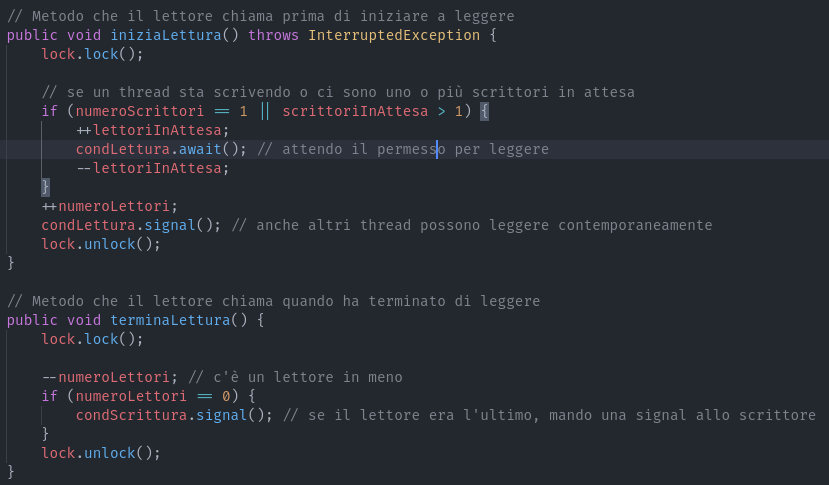
\includegraphics[width=0.52\linewidth]{img/monitor_lettore}
			\end{figure}
			
			
			\begin{figure}
				\centering
				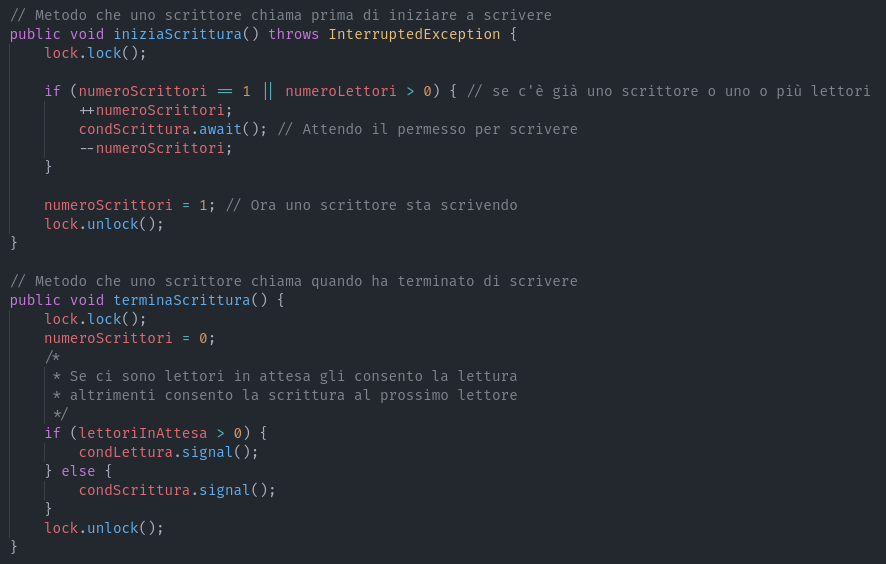
\includegraphics[width=0.52\linewidth]{img/monitor_scrittore}
			\end{figure}
			
\end{frame}

 %---Esecuzione Java----%
	\begin{frame}[fragile]
		\frametitle{Prima esecuzione}
		\begin{figure}
			\centering
			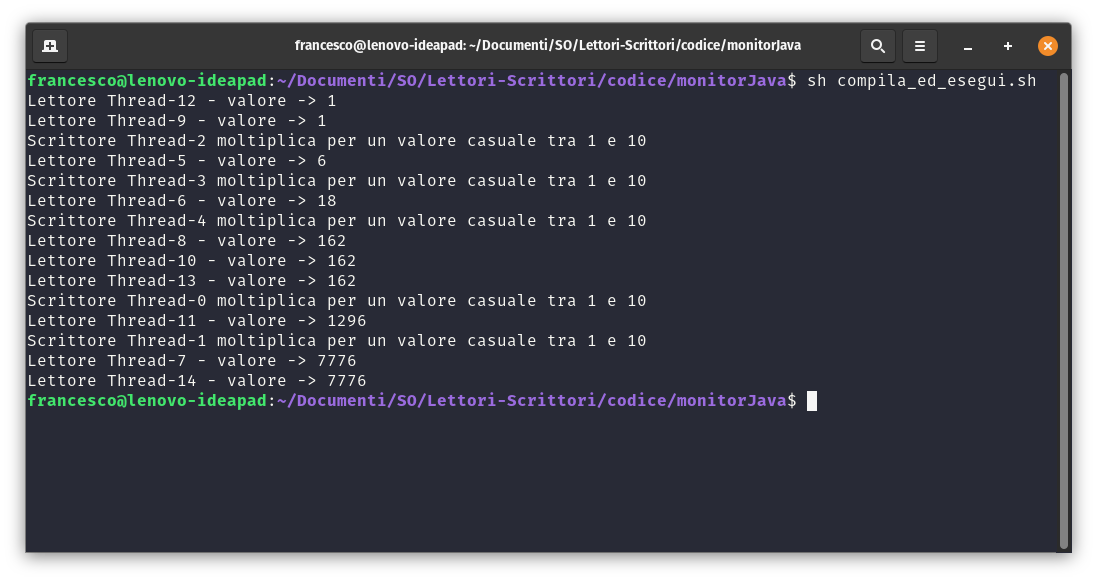
\includegraphics[width=1.03\linewidth]{img/esecuzione/programJ1}
		\end{figure}
	\end{frame}

	\begin{frame}[fragile]
		\frametitle{Seconda esecuzione}
		\begin{figure}
			\centering
			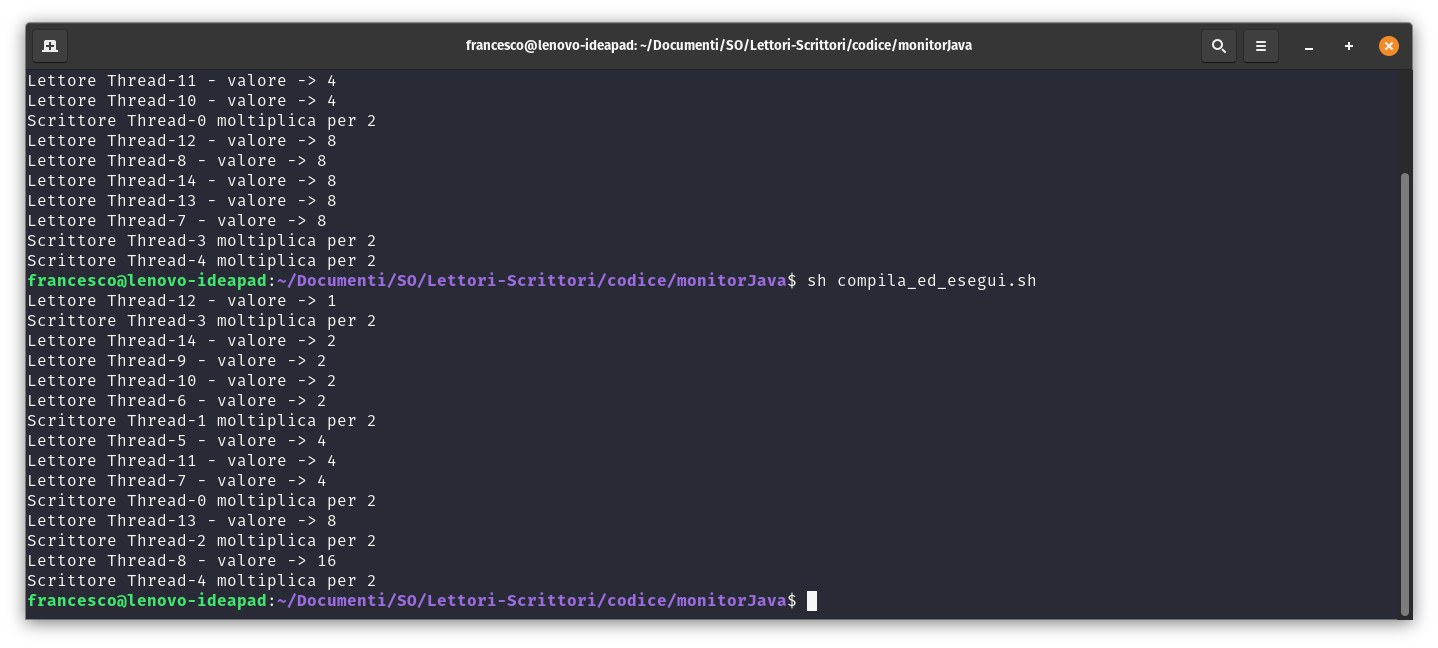
\includegraphics[width=1.03\linewidth]{img/esecuzione/programJ2}
		\end{figure}
	\end{frame}
	

	%------------------------------------------------
	
	%------------------------------------------------
	
	\begin{frame}
		\centerline{Link al repository con i sorgenti delle soluzioni viste e delle slides.}
		
		\centerline{\href{https://github.com/FrancescoLucia/Lettori-Scrittori.git}{https://github.com/FrancescoLucia/Lettori-Scrittori.git}}
	\end{frame}
	
	%----------------------------------------------------------------------------------------
	
\end{document} 